\documentclass[11pt,a4paper]{article}
\usepackage[T1]{fontenc}
\usepackage[utf8]{inputenc}
\usepackage[spanish,es-noshorthands]{babel}
\usepackage[margin=2.5cm]{geometry}
\usepackage{enumitem}
\usepackage{graphicx}
\graphicspath{{figs/}}
\setlist{itemsep=2pt}

\title{Hold delay scan del Citiroc con la CAEN A5202}
\author{}
\date{19 de octubre de 2026}

\begin{document}
\maketitle

\noindent Asumo que la tarjeta de lectura es una CAEN A5202 (dos Citiroc~1A, 64 canales),
controlada con el software Janus. Los nombres de los parámetros son los de
Janus (Sección~\ref{sec:janus}).

\section*{Programa de festejos}

\noindent {\bf Preparación, una vez}
\begin{itemize}
\item {\bf Acción:} montar sin cristal, con los fotomultiplicadores de
  silicio (SiPM) a oscuras y a 5~V de overvoltage. En Janus, poner los
  parámetros de la Sección~\ref{sec:janus} y además \texttt{OF\_ListCSV} = 1,
  \texttt{OF\_RunInfo} = 1, \texttt{OF\_ServiceInfo} = 1,
  \texttt{RunNumber\_AutoIncr} = 1, \texttt{StopRunMode} = PRESET\_COUNTS y
  \texttt{PresetCounts} = 20000.
\item {\bf Resultado:} cada run se para solo a los 20\,000 eventos y lleva su
  propio número \texttt{N}. Al acabar, Janus escribe en \texttt{DataFilePath}
  \texttt{RunN\_list.csv} (para cada evento y canal, la baja y la alta
  ganancia y el tiempo de llegada, time of arrival o ToA),
  \texttt{RunN\_Info.txt} (la configuración del run) y el fichero de
  temperatura y tensión.
\end{itemize}

\noindent {\bf Paso 1: staircase} (tasa de trigger frente al umbral)
\begin{itemize}
\item {\bf Acción:} lanzar la staircase de Janus con \texttt{OF\_Staircase} = 1.
\item {\bf Resultado:} Janus recorre \texttt{TD\_CoarseThreshold}, dibuja la
  tasa de trigger de cada canal frente al umbral y escribe
  \texttt{RunN\_Staircase\_0\_ch.txt} para cada canal.
\item {\bf Acción:} en la curva (Figura~\ref{fig:staircase}), elegir el valor
  del centro de la meseta de 1 fotoelectrón (pe), que corresponde a 0,5~pe
  (Sección~\ref{sec:umbral}), y ponerlo en \texttt{TD\_CoarseThreshold}.
\end{itemize}

\noindent {\bf Paso 2 (opcional): vistazo rápido}
\begin{itemize}
\item {\bf Acción:} lanzar el \texttt{Hold Delay Scan} de Janus con
  \texttt{Min} = 0, \texttt{Max} = 120, \texttt{Step} = 8 y \texttt{Nmean} =
  20000.
\item {\bf Resultado:} Janus dibuja, canal a canal, el espectro de alta
  ganancia frente al delay, pero no guarda nada. Sirve para ver dónde está
  el máximo antes de los runs buenos.
\end{itemize}

\noindent {\bf Paso 3: scan con el slow shaper (SS) de 25~ns}
\begin{itemize}
\item {\bf Acción:} \texttt{HG\_ShapingTime} = 25~ns y un run por cada
  \texttt{HoldDelay} = 0, 8, 16\ldots\ 120~ns: 16 runs, a mano o con Jobs
  (Sección~\ref{sec:janus}).
\item {\bf Resultado:} 16 ficheros \texttt{RunN\_list.csv}.
\item {\bf Acción:} el análisis de la Sección~\ref{sec:datos}: para cada run,
  la mediana sobre los canales de la posición y la anchura del pico de
  1~pe. Se elige el delay con la posición más alta. Si la posición es
  máxima en \texttt{HoldDelay} = 0 y disminuye a partir de ahí, el hold
  llega después del máximo del pulso incluso sin retraso añadido, y se
  repite el paso con SS de 50~ns (Sección~\ref{sec:th}).
\end{itemize}

\noindent {\bf Paso 4: scan con SS de 87,5~ns}
\begin{itemize}
\item {\bf Acción:} igual que el paso 3, con \texttt{HoldDelay} = 40, 48\ldots\
  160~ns (16 runs).
\end{itemize}

\noindent {\bf Qué necesita tu estudiante (servidor)}
\begin{itemize}
\item Todo lo que hay en \texttt{DataFilePath}.
\item Un registro, una línea por run: número de run, shaping,
  \texttt{HoldDelay}, overvoltage, \texttt{HG\_Gain},
  \texttt{TD\_CoarseThreshold}, eventos y temperatura.
\item Tu tabla de resultados de los pasos 3 y 4, con el delay elegido para
  cada shaping.
\end{itemize}

\section{Mecanismo}

\begin{figure}[htbp!]
\centering
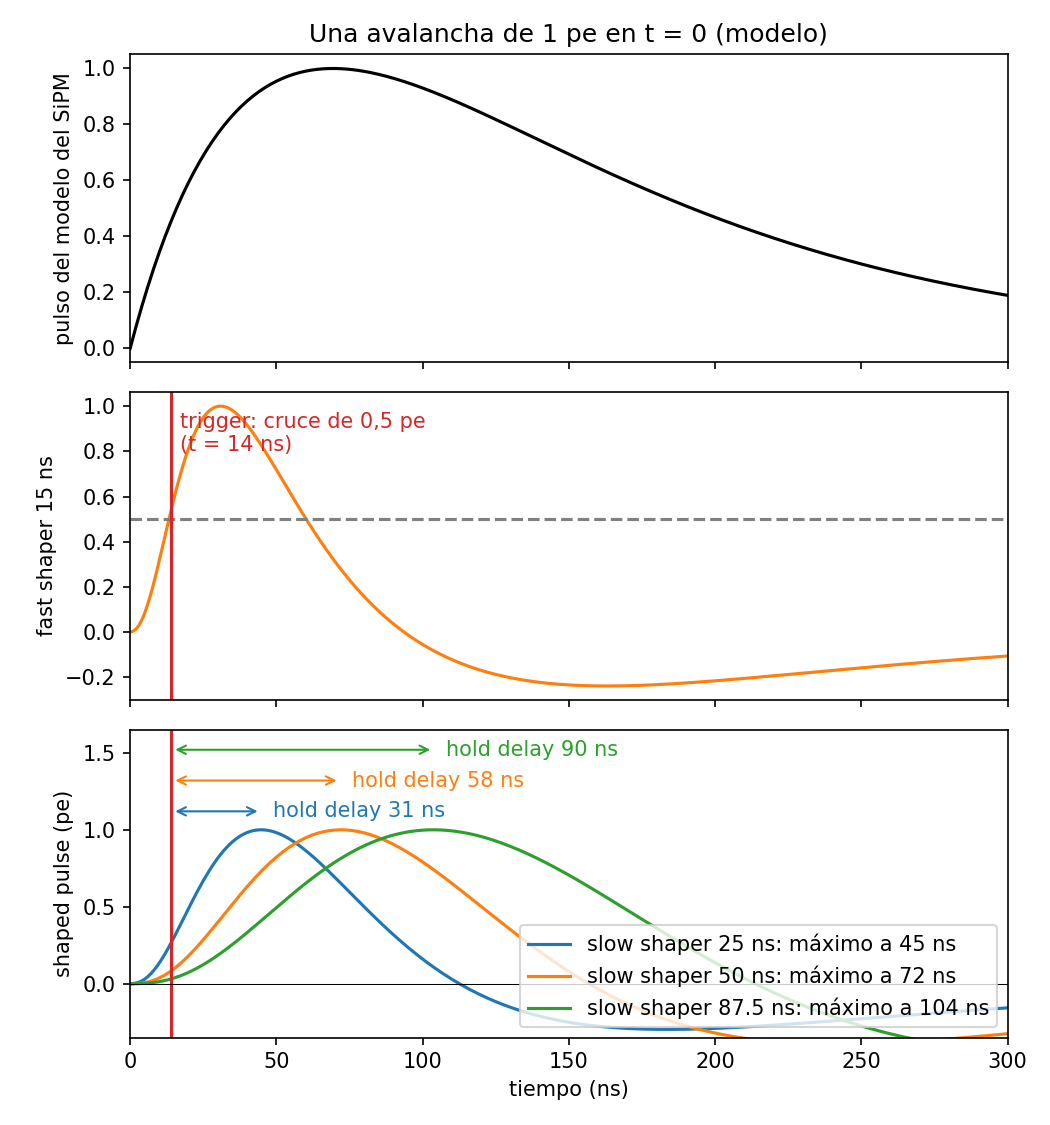
\includegraphics[width=0.75\textwidth]{mecanismo.png}
\caption{Una avalancha de 1~pe en $t = 0$, según el modelo de Montecarlo. {\bf Arriba}, el
pulso de una avalancha según el modelo del SiPM, normalizado a 1 en su
máximo. El pulso viene dado por la diferencia de dos exponenciales: la recarga de la celda
(del orden de 50~ns) y el producto de la capacitancia del SiPM con la
resistencia de entrada (2000~pF $\times$ 50~$\Omega$ = 100~ns). El pulso sube hasta su
máximo a 69~ns y cae con una constante de 100~ns. {\bf En el centro}, la salida del fast shaper: el trigger se produce cuando el pulso cruza 0,5~pe, a 14~ns. {\bf Abajo}, el pulso que sale del slow shaper a 25, 50 y
87,5~ns; el retraso (hold delay) que introduce el hold en su máximo es la
distancia entre el trigger y el máximo, 31, 58 y 90~ns, de acuerdo al modelo,
que no toma en cuenta retrasos asociados con la A5202 (board latency),
los cables, etc.}
\label{fig:mecanismo}
\end{figure}

El mecanismo se muestra en la Figura \ref{fig:mecanismo}. 

\begin{itemize}
\item Cada vez que se produce una avalancha en el SiPM (incluyendo los
  pulsos oscuros, dark pulses o DP, que usamos para la calibración), la señal (Fig. \ref{fig:mecanismo}, arriba)
  entra en el preamplificador de alta ganancia y pasa por el slow shaper (SS, que podemos
  fijar a 25~ns). De ahí sale un pulso de unas decenas de ns de ancho, con su
  máximo a una altura fija por pe (Fig. \ref{fig:mecanismo}, abajo).
\item En paralelo, el fast shaper (15~ns, FS) la compara con el umbral
  de 0,5~pe. Si lo cruza, el canal se dispara (da trigger; Fig. \ref{fig:mecanismo}, centro). En la A5202 el trigger del
  evento es el OR de los 64 canales de los dos chips, así que el hold es
  común a los 64 canales. El FS tiene que estar conectado a la alta
  ganancia.
\item La FPGA de la A5202 recibe el trigger y, pasado el hold delay, manda
  el hold. El hold delay se fija con el parámetro \texttt{HoldDelay} de Janus y solo
  puede valer un múltiplo de 8~ns, el periodo del reloj de la FPGA.
\item La cantidad que el chip digitaliza depende del peak sampling mode
  (track \& hold o peak detector, Sección~\ref{sec:modos}).
\end{itemize}

\section{Track \& hold vs peak detector}
\label{sec:modos}

El peak sampling mode se elige con el parámetro \texttt{PeakDetectorMode} que toma dos valores:
PEAK\_STRETCH (peak detector, el valor por defecto) o TRACK\&HOLD. Se
aplica a las dos ganancias a la vez.

\begin{itemize}
\item {\bf Track \& hold:} guarda el valor de la señal en el instante del
  hold. Es el modo que usa la simulación para la calibración con espectros
  de un fotoelectrón (single photoelectron, SPE), y la
  A5202 lo permite. Hay que comprobar que la latency de la A5202 no pase ya
  el máximo del pulso con SS de 25~ns (Sección~\ref{sec:th}). En ese caso usaríamos un SS más largo. 
\item {\bf Peak detector:} guarda el máximo entre el trigger y el hold, así
  que el delay es la longitud de una ventana. Es el modo adecuado para la
  medida de energía pero no el mejor para los SPE.
\end{itemize}

Para la calibración se usa {\bf track \& hold} (Sección~\ref{sec:th}).

\section{Razón de la medida}

\begin{itemize}
\item Queremos que el valor guardado sea el máximo del pulso a la salida
  del SS. Esa altura es la unidad de calibración: el modelo de
  simulación representa la luz que guarda el Citiroc como fracción de ese
  máximo.
\item En track \& hold, si el hold cae fuera del máximo, el valor guardado
  es menor (la ganancia sale baja) y varía de una avalancha a otra. El
  instante del trigger cambia un poco según la amplitud y el ruido, y en la
  pendiente del pulso eso se traduce en amplitud, así que los picos se
  ensanchan. En el máximo la pendiente es nula y el efecto desaparece.
\item El modelo simulado pasa una sola avalancha de 1~pe, sin ruido, por la
  simulación del preamp del Citiroc, del FS y del SS
  (Figura~\ref{fig:mecanismo}): el FS da el instante del trigger, cuando la
  señal cruza el umbral de 0,5~pe, y el SS el instante de su máximo.
\item La diferencia entre los dos instantes es el delay. El modelo predice
  31~ns a 25~ns de shaping, 58~ns a 50~ns y 90~ns a 87,5~ns. La cuenta se
  deja cositas sin modelar: no incluye retrasos en la A5202 o los cables y
  asume una forma de pulso para la SPE que puede ser un poco diferente de la
  real. De ahí la necesidad de hacer un scan.
\end{itemize}

\begin{figure}[htb]
\centering
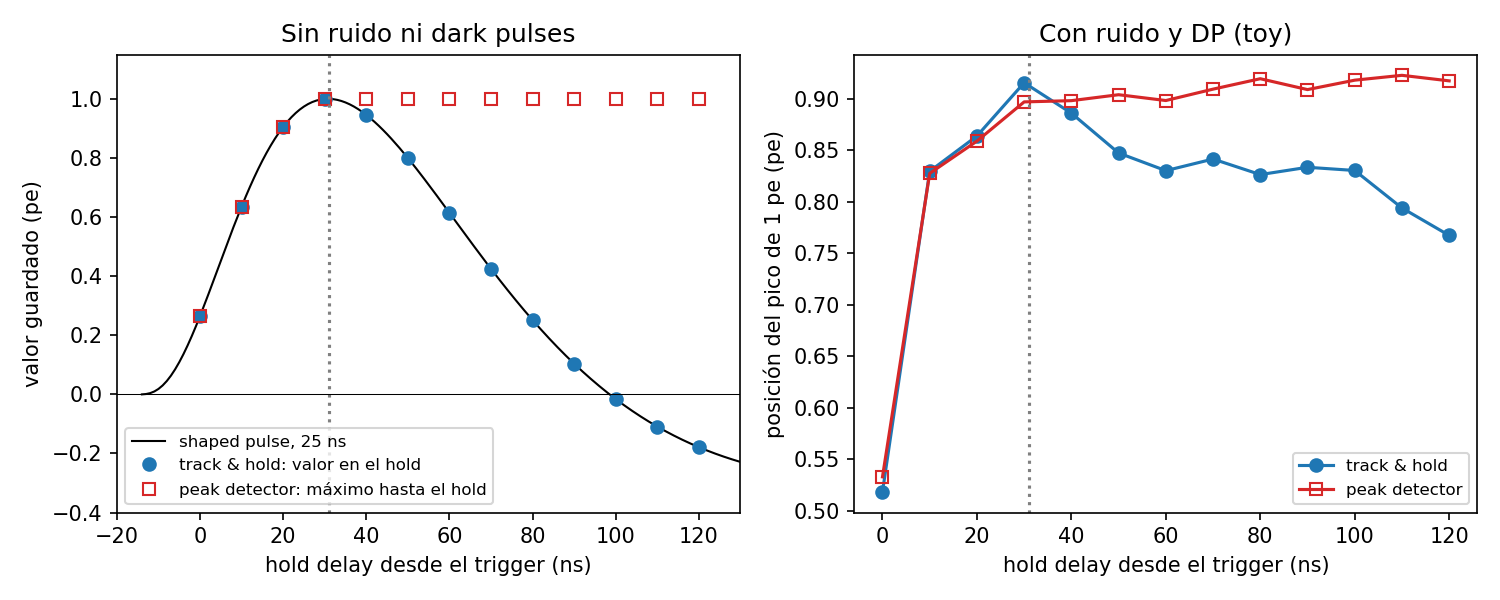
\includegraphics[width=\textwidth]{modos.png}
\caption{Valor guardado frente al hold delay, shaping de 25~ns. Izquierda,
una avalancha sola: en track \& hold el valor sigue el shaped pulse (los
puntos dibujan su forma), en peak detector sube hasta el máximo y se queda
en él. Derecha, la posición del pico de 1~pe en un toy con ruido, DP a
4,4~MHz y crosstalk del 19,5\% (5~V): la misma pauta, con el pico
algo por debajo de 1 por el pile-up. La línea de puntos marca el delay del
modelo, 31~ns.}
\label{fig:modos}
\end{figure}

\begin{figure}[htb]
\centering
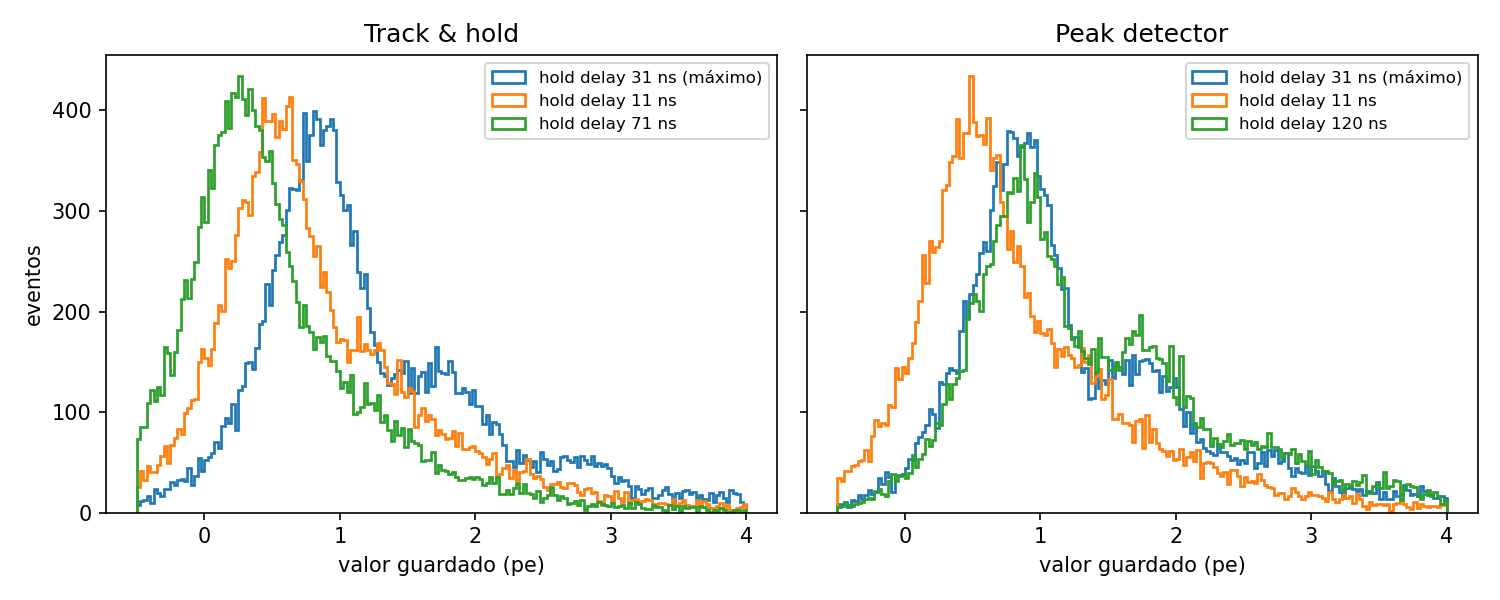
\includegraphics[width=\textwidth]{espectros.png}
\caption{Espectros del toy de la Figura~\ref{fig:modos} para tres hold
delays. En track \& hold, fuera del máximo (11 y 71~ns) los picos se
desplazan hacia abajo y se borran; en el máximo (31~ns) se ven los picos
de 1, 2 y 3~pe. En peak detector, un delay corto (11~ns) corta la subida
del pulso; 31 y 120~ns dan casi el mismo espectro.}
\label{fig:espectros}
\end{figure}

\section{Parámetros de Janus (A5202)}
\label{sec:janus}

\begin{center}
\small
\begin{tabular}{p{0.3\textwidth} p{0.6\textwidth}}
\hline
parámetro & valor para los runs SPE \\
\hline
\texttt{AcquisitionMode} & SPECT\_TIMING: además del valor ADC guarda el tiempo de
llegada (ToA) de cada canal que disparó \\
\texttt{BunchTrgSource} & T-OR (OR de los time discriminators) \\
\texttt{TriggerLogic} & OR64 \\
\texttt{FastShaperInput} & HG-PA (FS en la alta ganancia) \\
\texttt{TD\_CoarseThreshold} & el que corresponde a 0,5~pe (Sección~\ref{sec:umbral}) \\
\texttt{PeakDetectorMode} & TRACK\&HOLD \\
\texttt{HoldDelay} & el del scan, múltiplo de 8~ns \\
\texttt{HG\_ShapingTime} & el del scan (25, 50 o 87,5~ns) \\
\texttt{LG\_ShapingTime} & 87,5~ns \\
\texttt{HG\_Gain} & alto (de 1 a 63); si los picos de 1~pe no se separan del
pedestal, subirlo antes que el overvoltage \\
\texttt{GainSelect} & BOTH \\
\texttt{StopRunMode}, \texttt{PresetCounts} & PRESET\_COUNTS, 20000: cada run
para solo a los 20k eventos \\
\texttt{OF\_ListCSV}, \texttt{OF\_RunInfo}, \texttt{OF\_ServiceInfo} & 1 (los
ficheros del resumen ejecutivo) \\
\texttt{OF\_Staircase} & 1 en el run de la staircase \\
\hline
\end{tabular}
\end{center}

\noindent Janus tiene un hold delay scan propio (\texttt{Hold Delay Scan}: \texttt{Min}, \texttt{Max},
\texttt{Step} múltiplo de 8~ns, \texttt{Nmean} eventos por paso). Dibuja, para cada canal, el
espectro de alta ganancia frente al delay, pero no guarda los datos y no
separa los canales que dispararon. Sirve para un primer vistazo, con \texttt{Nmean}
de al menos 20\,000; el delay se elige con los runs de la
Sección~\ref{sec:th}, que sí se guardan.

Los 32 runs de los scans se pueden encadenar con el modo Jobs de Janus
(\texttt{EnableJobs} = 1, \texttt{JobFirstRun}, \texttt{JobLastRun}): para cada
número de run Janus carga su propio fichero de configuración,
\texttt{Janus\_Config\_RunN.txt}, que solo difiere en \texttt{HoldDelay} y,
en su caso, en \texttt{HG\_ShapingTime}.

\section{Datos y análisis}
\label{sec:datos}

\begin{itemize}
\item {\bf Datos:} en cada run la adquisición guarda, en cada evento, el
  valor ADC de los 64 canales y, en SPECT\_TIMING, el ToA de cada canal que
  disparó.
\item {\bf Análisis:} para cada canal, el espectro con los eventos en que
  fue el primero en disparar, según los ToA. Muestra el pedestal y los
  picos de 1, 2 y 3~pe. Para cada canal se ajusta una gaussiana al
  pedestal y otra al pico de 1~pe, cada una en una ventana alrededor de su
  máximo. La posición del pico de 1~pe es la diferencia entre las dos
  medias, en ADC counts, y su anchura es la sigma de la segunda gaussiana.
  Para comparar delays se usa la mediana sobre los 64 canales de la
  posición y de la anchura. Si en un evento disparan varios canales, el hold,
  común a los 64 canales, se cuenta desde el primero, y los demás quedan medidos
  fuera de su máximo.
\item {\bf Estadística:} 20k eventos por run. Con el OR de 64 canales cada
  canal es el primero en unos 300 eventos, que miden la posición del pico de
  1~pe al 0,6\%. Con eso, deberíamos encontrar el delay.
\end{itemize}


\begin{figure}[htbp!]
\centering
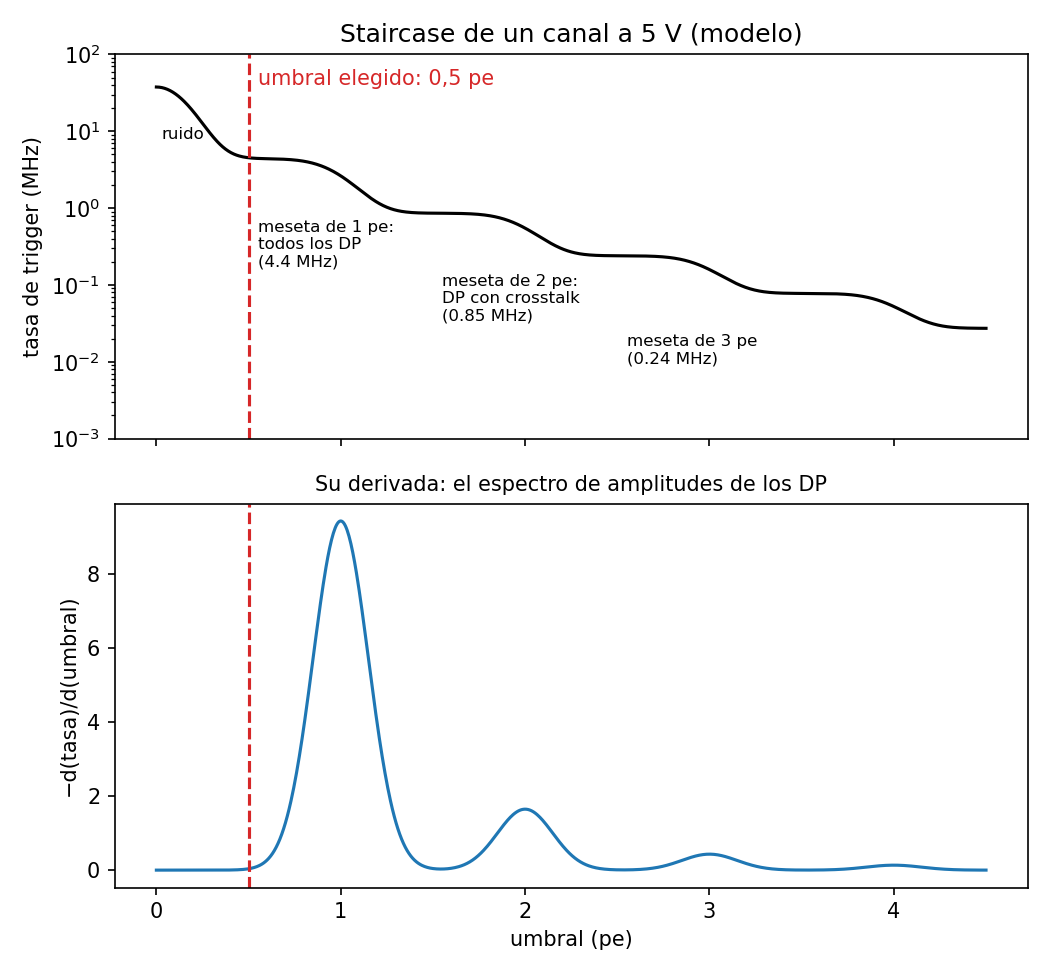
\includegraphics[width=0.75\textwidth]{staircase.png}
\caption{Staircase de un canal a 5~V según el modelo: DP a 4,4~MHz,
crosstalk del 19,5\% y ruido de 0,15~pe en el FS. Arriba, tasa de trigger
frente al umbral, en pe; en los datos el eje es el valor de
\texttt{TD\_CoarseThreshold}. Abajo, su derivada, el espectro de amplitudes
de los DP. La línea roja marca el umbral elegido.}
\label{fig:staircase}
\end{figure}


\section{Determinación del umbral antes del scan}
\label{sec:umbral}

El trigger tiene que dispararse con 0,5~pe, pero la A5202 no trae el umbral
en pe: \texttt{TD\_CoarseThreshold} es un valor de DAC (220 por defecto),
común a los 32 canales de cada chip, y lo que vale en pe depende de
\texttt{HG\_Gain}, del overvoltage y de la forma del pulso. Por eso, antes del
scan, se fija con la staircase de Janus.

\begin{itemize}
\item {\bf Qué hace:} Janus recorre \texttt{TD\_CoarseThreshold} (por defecto
  de 150 a 300 en pasos de 1, 500~ms por paso) y mide la tasa de trigger de
  cada canal. 
\item {\bf Qué obtenemos} (Figura~\ref{fig:staircase}, arriba): con los
  SiPMs a oscuras, la tasa de trigger frente al umbral baja en escalones.
  Con el umbral dentro del ruido electrónico la tasa es enorme. Entre el
  ruido y 1~pe la tasa es casi constante: es la meseta de 1~pe. Ahí dispara
  cualquier DP, así que la tasa es la de cuentas oscuras, unos 4,4~MHz por
  canal a 5~V según el modelo. Por encima de 1~pe solo disparan los DP que
  encienden al menos otra celda por crosstalk: es la meseta de 2~pe, unas
  cinco veces más baja (crosstalk del 19,5\%). Y así sucesivamente. La
  derivada de la curva (Figura~\ref{fig:staircase}, abajo) es el espectro de
  amplitudes de los DP: el umbral de 0,5~pe cae en el valle entre el ruido y
  el pico de 1~pe.
\item {\bf Qué valor buscamos:} el valor en el centro de la meseta de 1~pe, a
  medio camino entre el borde del ruido y el escalón de 1 a 2~pe. Eso es
  0,5~pe. Si los canales no coinciden, se toma el valor que deja a todos
  dentro de su meseta.
\item {\bf Condiciones:} las del scan (5~V, \texttt{HG\_Gain} elegido,
  \texttt{FastShaperInput} = HG-PA). Si cambian el overvoltage o
  \texttt{HG\_Gain}, hay que repetirla.
\item {\bf De propina:} la altura de las mesetas da la tasa de cuentas
  oscuras y el crosstalk, que se comparan con el modelo.
\end{itemize}



\section{Instrucciones con track \& hold}
\label{sec:th}

\begin{itemize}
\item \texttt{PeakDetectorMode} = TRACK\&HOLD, 5~V, umbral de 0,5~pe, shaping
  de 25~ns en alta ganancia.
\item Hold delay de 0 a 120~ns en pasos de 8~ns, un run por paso.
\item Elegimos el delay con la posición más alta del pico de 1~pe
  (Sección~\ref{sec:datos}), que debe
  coincidir con la anchura mínima. Ese delay se usa en todos los runs SPE
  con shaping de 25~ns.
\item Comprobación de la latency: el trigger sale del chip, pasa por la FPGA
  y vuelve como hold, con un retraso fijo que se suma al \texttt{HoldDelay}. Si la
  posición del pico de 1~pe es máxima en \texttt{HoldDelay} = 0 y disminuye a
  partir de ahí, ese retraso ya ha pasado el máximo del pulso. En ese caso se repite el scan
  con SS de 37,5 o 50~ns, cuyo máximo llega más tarde (58~ns a 50~ns, según
  el modelo), y ese shaping pasa a ser el de la calibración.
\item Se repite con shaping de 87,5~ns, con el hold delay de 40 a 160~ns en
  pasos de 8~ns.
\end{itemize}

\noindent Resultado (esperado):
\begin{itemize}
\item El hold delay correcto para la calibración.
\item La forma del shaped pulse. Cada run guarda el pulso en un solo
  instante, el hold delay, y la posición del pico de 1~pe es la amplitud del
  pulso en ese instante. La posición del pico frente al delay nos da el
  pulso de una avalancha, punto a punto (Figura~\ref{fig:modos},
  izquierda), y nos permite calibrar el modelo.
\end{itemize}

\end{document}
